\documentclass{article}

\usepackage[english]{babel}
\usepackage[utf8]{inputenc}
\usepackage{amsmath,amssymb}
\usepackage{tabularx}
\usepackage{booktabs}
\usepackage{enumitem}
\usepackage{parskip}
\usepackage{graphicx}

\usepackage[top=2.5cm, left=3cm, right=3cm, bottom=4.0cm]{geometry}

\newcommand{\lectureheader}[4]{%
  \begin{minipage}{.3\textwidth}%
    
    \strut
\includegraphics[width=\textwidth]{figures/ethlogo.pdf}%
  \end{minipage} \hfill%
  \raisebox{1.5mm}{%
    \begin{minipage}{0.69\textwidth}\sf\flushright%
        \textbf{\Huge #3}\mbox{\hspace{2mm}}\\#4\mbox{\hspace{2mm}}%
    \end{minipage}%
  }\\[-2mm]\hrule%
  \begin{minipage}[t]{0.5\textwidth}\sf\textit{#1} \end{minipage} \hfill%
  \begin{minipage}[t]{0.5\textwidth}\sf\flushright \textit{#2}\end{minipage}%
  \par%
}

% Create commands for syntax that you will frequently use
\newcommand{\xx}{\mathbf x}

\begin{document}
\begin{titlepage} 

\lectureheader{Prof. Ryan Cotterell}
{}
{\Large Natural Language Processing}{Spring 2021}
	\newcommand{\HRule}{\rule{\linewidth}{0.5mm}} 
	
	\center % Centre everything on the page
	{\Huge Course Assignment}\\
      \quad\newline
	
	{\large\today} \\
	\quad\newline
	%	Author
	%------------------------------------------------
	
	{\Large Firstname Lastname \\ \emph{nethz} Username: ryancotterell \\ Student ID: 00000000}\\[0.5cm] 
	\vfill
	{\large \textbf{Collaborators:} \\
	Other student 1 \\
	Other student 2}
	
	\vfill\vfill\vfill 
	By submitting this work, I verify that it is my own. That is, I have written my own solutions to each problem for which I am submitting an answer. I have listed above all others with whom I have discussed these answers.
	
	\vfill 
	
\end{titlepage}

%%%%%%%%%%%%%%%%%
%   Problem 1   %
%%%%%%%%%%%%%%%%%
\section*{Problem 1}
\begin{enumerate}[label = (\alph*)]
    \item The problem states that we should find $x$ that solves the following equation
\begin{align}
    \label{eq:example_equation} % Equation label; can be used for referencing
    2 x^2 + 4 x - 6 = 0 \,.
\end{align}
\begin{enumerate}[label = (\roman*)]
    \item We take the standard algorithm for solving equations of the form $a x^2 + bx + c$ and apply it to Equation~\ref{eq:example_equation}. This gives us
\begin{align}
    x 
    &= \frac{2}{2 \cdot 2} \pm \sqrt{\left( \frac{2}{2 \cdot 2} \right)^2 + \frac{6}{2} } \\
    &= 1 \pm 2
\end{align}
So the solutions are $x=3$ and $x = -1$.
\end{enumerate}
\item Example of how to add figure (can be used for jpeg, png, pdf, eps etc)
In Figure~\ref{fig:roller-coaster}, we can see an example of how people in our class must feel.
\begin{figure}[h!]
    \centering
    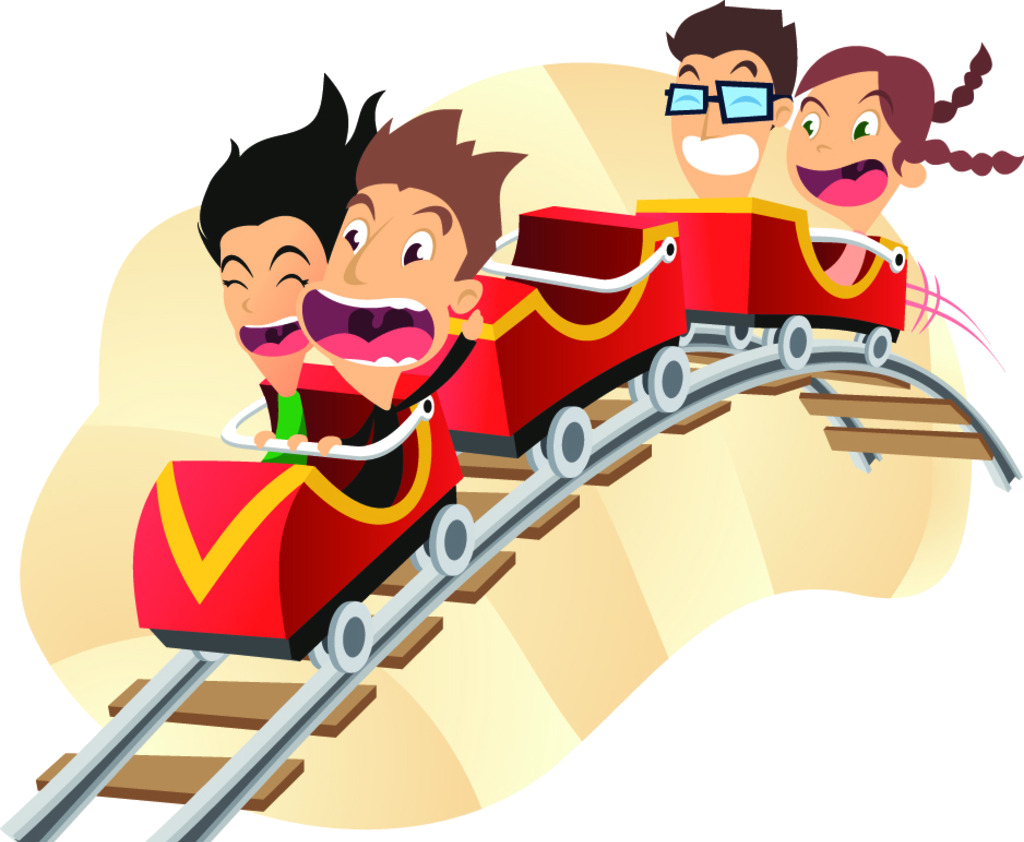
\includegraphics[scale=0.2]{figures/roller-coaster.png}
    \caption{Example figure}
    \label{fig:roller-coaster}
\end{figure}
\end{enumerate}






%%%%%%%%%%%%%%%%%
%   Problem 2   %
%%%%%%%%%%%%%%%%%
\pagebreak
\section*{Problem 2}

Example of simple, centered table:

\begin{table*}[h!]
\centering
    \begin{tabular}{c | llllll }
        \toprule
         BV  & z & $x_1$ & $x_2$ & $x_3$ & $x_4$ & $x_5$  \\ 
         \midrule % horizontal line
         $y_1$   & 1 & 0 & 0 & $-\frac{2}{5}$ & -$\frac{1}{5}$ & 0  \\
         $y_2$ & 0 & 0 & 1 & $-\frac{1}{5}$ & $\frac{2}{5}$  & 0  \\
        \bottomrule
    \end{tabular}
\end{table*}



Here is how you make vectors and matrices:
\begin{align}
    \xx = \begin{bmatrix} 1 & 2 & 3 \end{bmatrix} = \begin{bmatrix} 1 \\ 2 \\ 3 \end{bmatrix}^\top \\
    A = \begin{bmatrix} 1 & 2 & 3 \\ 4 & 5 & 6 \end{bmatrix}^{-1}
\end{align}

Since I use the formula $\mathbf x$ often, I have created a macro for it in the header of this document such that I can use $\xx$ for shorthand.

Here is a formulation of a linear program:
\begin{align}
    \min_{x} \quad & c^\top x \\
    \mathrm{s.t.} \quad 
    & A x \leq b \\
    &-1 \leq x_n \leq 1 \,, \quad n = 1, \dots, N
\end{align}

\clearpage
\newpage

\begin{table}[h]
        \centering
        \fontsize{10}{10}\selectfont
        \renewcommand{\arraystretch}{1.2} % vertical padding
        \setlength{\tabcolsep}{0.5em} % for the horizontal padding
        \begin{tabular}{l|l|l|l}
        \textbf{number} & \textbf{sample strings} & \textbf{accepted} & \textbf{weight} \\ \hline
        1 & educational is this not &  &  \\
        2 & is this assignment educational &  &  \\
        3 & not educational is not educational &  &  \\
        4 & this assignment is not educational &  &  \\
        5 & is this assignment educational &  &  \\
        6 & this assignment course is educational &  &  \\
        7 & is this assignment not educational &  &  \\
        8 & this assignment not &  &  \\
        9 & this course assignment is not educational &  &  \\
        10 & this course is not not educational &  &  \\
        11 & not educational is this &  &  \\
        12 & course assignment is not educational &  &  \\
        13 & not this assignment is educational &  &  \\
        14 & not not not educational &  &  \\
        14 & is this course assignment not educational &  &  \\
        15 & course assignment is this &  &  \\
        16 & this course is interesting &  &  \\
        17 & this course assignment not educational &  & 
        \end{tabular}
        \caption{Some strings from $\mathcal{Y}_{\geq 2, \leq 6}$}
        \label{tab:wfst_strings}
        \end{table}
        
\begin{figure}[!h]
        \centering
        \includegraphics[width=1.0\textwidth]{./figures/wfst_charts_1.pdf}
        % \includegraphics[width=.45\linewidth]{./fig/C1000.png}
        \caption{Floyd-Warshall algorithm, iteration 0 to 3; left column matrix should contain weights after iteration n; right column matrix should be iteratively filled for backtracking each path}
        \label{fig:wfst_charts_1}
    \end{figure} 
    
    \begin{figure}[!h]
        \centering
        \includegraphics[width=1.0\textwidth]{./figures/wfst_charts_2.pdf}
        % \includegraphics[width=.45\linewidth]{./fig/C1000.png}
        \caption{Floyd-Warshall algorithm, iteration 4 to 7; left column matrix should contain weights after iteration n; right column matrix should be iteratively filled for backtracking each path}
        \label{fig:wfst_charts_2}
    \end{figure} 
\end{document}
